A obtenção do modelo matemático resulta em uma equação conforme segue.
Os detalhes do equacionamento podem ser acompanhados no Anexo B.
A Equação \ref{eq:resultadoModelo}, no formato canônico,  mostra a constante de tempo $\tau
= 2,5s$, para o sistema de primeira ordem utilizado neste estudo.  

\begin{equation}
  \frac{C(s)}{R(s)} = \frac{1}{\tau s+1} = \frac{1}{2,5 s+1}
\label{eq:resultadoModelo}
\end{equation}

Na Figura \ref{fig:resultadoft} pode ser visualisada a 
escala de tempo devidamente ajustada para um intervalo de mesmo
valor da constante de tempo $\tau$, facilitando a interpretação do
sinal aquisitado.

\begin{figure}[!htb]
\centering
\caption{Resultado gráfico do modelo matemático}
\center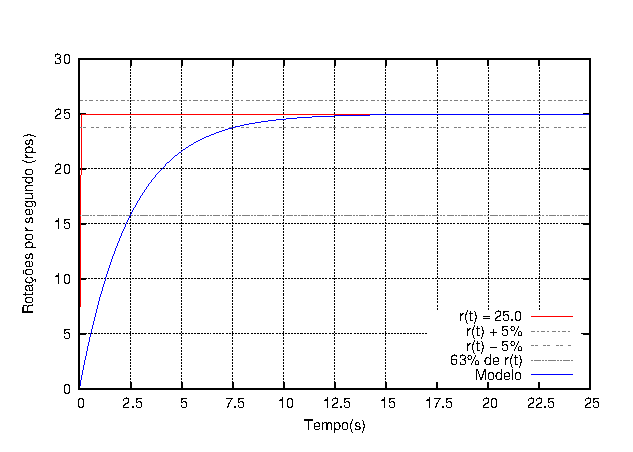
\includegraphics[scale=1.3]{./plot/ft.eps}

\label{fig:resultadoft}

{\small Fonte: Próprio autor}
\end{figure}



Ao aquisitar a curva de acionamento do sistema em malha aberta,
constuindo o gráfico das curvas aquisitada e calculada juntas  temos o
que é mostrado na Figura \ref{fig:resultadoMalhaAberta}:


\begin{figure}[!htb]
\centering
\caption{Comparação do modelo matemático com o comportamento empírico}
\center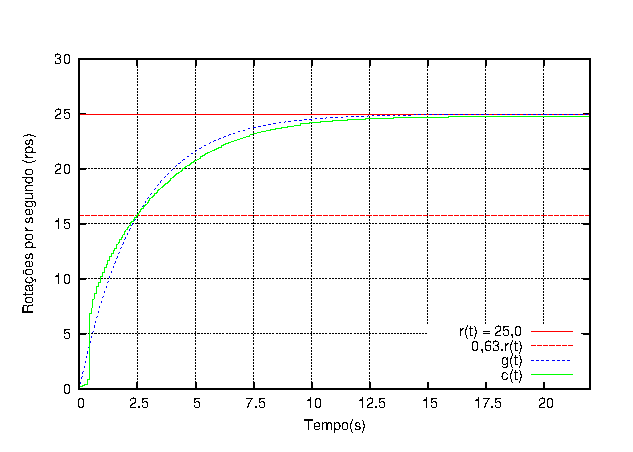
\includegraphics[scale=1.3]{./plot/acaoMalhaAbertaTau.eps}

\label{fig:resultadoMalhaAberta}

{\small Fonte: Próprio autor}
\end{figure}

Realizando a somatória para o cálculo de erro médio com todas as amostras aquisitadas: 

\begin{equation}
 \% erro = \frac{100}{N} . \sum_{n = 0,00}^{n=22,40} {\frac{| \text{\emph{r[n]}} -\text{\emph{c[n]}} |}{\text{\emph{r[n]}}} } 
\end{equation}


Onde:

\setlength{\parindent}{2cm}
r : valor real; 

c : valor calculado;

n : número da amostra aquisitada;

N : número total de amostras.

Obs.: As aquisições começaram com tempo inicial de 0,00 s até o tempo final de 22,40 segundos, com intervalo de 10 milisegundos entre aquisições, totalizando 2240 amostras.

\setlength{\parindent}{1cm}


Foi obtido um valor médio de 2,71\% de erro 
para o intervalo de aquisição de 50ms até os 22,40 s, 
que é o fim da aquisição, 
desconsiderando a região transitória não linear 
que ocorre nos instantes iniciais, 
mas que considera-se não relevante para a atual análise, 
inclusive pelo baixo valor de erro no restante do intervalo de comparação.


De forma mais detalhada, 
foram calculados os erros médios relativos para cada intervalo de 
tempo de um $\tau$, 
e pode-se notar, 
pela Tabela \ref{tab:resultadoErroModeloTau}, 
que o erro de estado estacionário, para o intervalo acima de 5 $\tau$, é menor do que 1\%. 


\begin{table}[h]
\centering
\caption{Erro Relativo Percentual para intervalos determinados por $\tau$ }
\label{tab:resultadoErroModeloTau}

\begin{tabular}{c|c}
\hline
Intervalo de amostras  &  erro médio relativo \\ \hline
\hline
%0 a 1 $\tau$ & 83,40 \% \\ \hline
1 a 2 $\tau$ &  3,16 \% \\ \hline
2 a 3 $\tau$ &  3,38 \% \\ \hline
3 a 4 $\tau$ &  2,00 \% \\ \hline
4 a 5 $\tau$ &  2,29 \% \\ \hline
$>$ 5 $\tau$ &  0,82 \% \\ \hline
\end{tabular}

{\vspace{0.2cm} \small Fonte: Próprio autor}
\end{table}

Desconsiderando a região transitória não linear 
que ocorre nos instantes iniciais do movimento do eixo do motor, 
o intervalo de maior erro é de 3,38\%, 
conforme mostrado na Tabela \ref{tab:resultadoErroModeloTau},
ressaltando ainda que no regime estacionário 
o erro é menor do que 1\%.
Assim, considera-se que o modelo utilizado é bom e representa razoavelmente bem o sistema físico real.

A Figura \ref{fig:resultadoAcaoPILPAEt} mostra de forma sobreposta os
resultados, em forma gráfica, para um sinal de referência do tipo
degrau e com valor em 25 rps, sendo acompanhado por linhas tracejadas
nos valores de tolerância de  $\pm 5\%$, bem como o comportamento da
planta em malha aberta, para que se possa ter uma melhor dimensão
do comportamente nos ensaios utilizando os controles PI e LPA$E\tau$ com diagrama Pereira-Leão.
A grade de apresentação do gráfico foi mantida com intervalo de 2,5s para o
período, mantendo cada unidade igual a um $\tau$. 





\begin{figure}[!htb]
\centering
\caption{Resultado dos controladores PI e LPA$E\tau$}
\center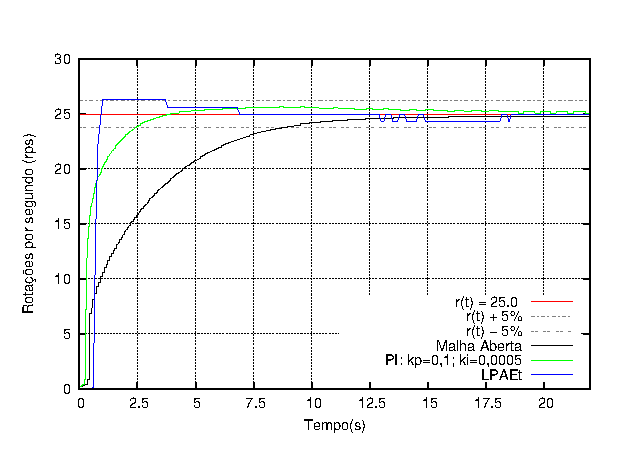
\includegraphics[scale=1.6]{./plot/resAcaoPI.eps}
\label{fig:resultadoAcaoPILPAEt}

{\small Fonte: Próprio autor}
\end{figure}









A resposta obtida para o sistema estudado pode ser vista na Figura \ref{fig:resultadoAcaoPILPAEt} onde podem ser destacados os seguintes pontos:

\begin{itemize}
\item No momento inicial, há um atraso de resposta devido à inércia do
  sistema físico, porém ao vencer esta condição inicial a velocidade
  de regime é alcançada rapidamente, em um tempo pouco menor do que $\frac{1}{2}$ do valor da constante de tempo $\tau$ do modelo do sistema.

\item O sobressinal apresentado alcança um valor ligeiramente acima da
  indicação superior de $5\%$ do valor de referência, metade do limite máximo aceitável de acordo com os requisitos de desempenho do sistema.

\item O sistema utilizando um controle PI entra em regime no tempo de
  2,5s, enquanto que para o controlador LPA$E\tau$ o regime é
  alcançado com um tempo de 3,75s, considerando que o sobressinal
  ligeiramente acima dos $5\%$ não é aceito para a janela do sistema
  em regime. Se tal valor for considerado e aceitável, o controlador
  LPA$E\tau$ entra em regima com um tempo de 1,75s aproximadamente.
Para o sistema em malha aberta o regime é alcançado com tempo de 8,75s. 

\end{itemize}


A Tabela \ref{tab:resultadoComparaErros}
mostra o erro médio relativo do
resultado dos dois controladores.
Em função do tempo de resposta
inicial, para esta tabela foi utilizado um intervalo de um segundo para gerar as amostras.

Um destaque pode ser dado aos dois primeiros intervalos de amostra,sendo que cada controlador obteve melhor desempenho em um deles.




\begin{table}[h]
\centering
\caption{Erro Médio Relativo Percentual }
\label{tab:resultadoComparaErros}


\begin{tabular}{c|c|c}
\hline
Intervalo de amostras  &  Controle PI &
Controle LPA$E\tau$ \\ \hline
\hline
 0 a  1 s & 50,57 \% &  75,68 \% \\ \hline
 1 a  2 s & 13,50 \% &  -5,20 \% \\ \hline
 2 a  3 s &  5,48 \% &  -5,20 \% \\ \hline
 3 a  4 s &  1,62 \% &  -4,64 \% \\ \hline
 4 a  5 s &  0,10 \% &  -2,40 \% \\ \hline
 5 a  6 s & -0,65 \% &  -2,40 \% \\ \hline
 6 a  7 s & -1,19 \% &  -2,16 \% \\ \hline
 7 a  8 s & -1,62 \% &   0,00 \% \\ \hline
 8 a  9 s & -1,78 \% &   0,00 \% \\ \hline
 9 a 10 s & -1,78 \% &   0,00 \% \\ \hline
10 a 11 s & -1,64 \% &   0,00 \% \\ \hline
11 a 12 s & -1,31 \% &   0,00 \% \\ \hline
12 a 13 s & -0,96 \% &   0,00 \% \\ \hline
13 a 14 s & -0,87 \% &   1,40 \% \\ \hline
14 a 15 s & -0,58 \% &   1,68 \% \\ \hline
15 a 16 s & -0,50 \% &   2,80 \% \\ \hline
16 a 17 s & -0,18 \% &   2,80 \% \\ \hline
17 a 18 s & -0,28 \% &   2,80 \% \\ \hline
18 a 19 s &  0,00 \% &   0,84 \% \\ \hline
19 a 20 s &  0,21 \% &   0,00 \% \\ \hline

\end{tabular}

{\vspace{0.2cm} \small Fonte: Próprio autor}
\end{table}




O primeiro intervalo de amostras (0 a 1s),
o controle PI obtem um resultado melhor,
pois apresenta um erro,
apesar de muito elevado,
muito menor do que o controlador LPA$E\tau$.
O segundo intervalo de amostras (1 a 2s),
pode-se notar que o erro está menor do que o
requisito de desempenho para este sistema
para o controlador LPA$E\tau$,
mas ainda não atingiu o mesmo limiar com
o controlador PI.  

O restante dos intervalos apresentam resultado satisfatório pois
apresentam-se dentro dos requisitos de desempenho do sistema, em ambos
os controles.













%\begin{figure}[!htb]
%\caption{Controle utilizando LPAE$\tau$}
%\center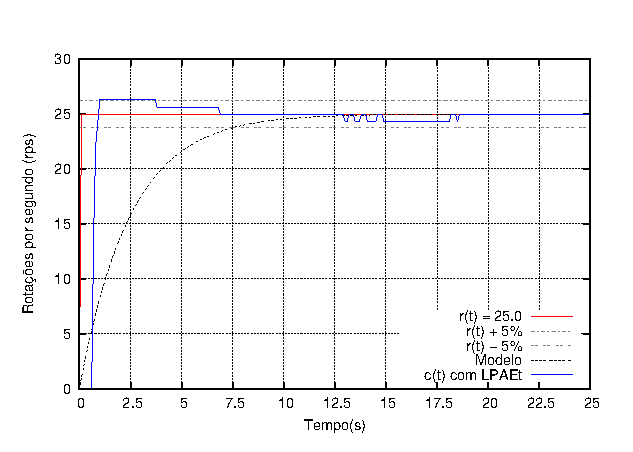
\includegraphics[scale=1.4]{./imagens/a3.eps}
%\label{fig:lpaet}

%{\small Fonte: Próprio autor}
%\end{figure}

%Todos os requisitos de desempenho do sistema foram atendidos, cumprindo com o objetivo inicial como pode-se ver na Figura \ref{fig:lpaet}. 





\section{Outros testes realizados}

Alguns testes foram realizados para validar a aplicação do $\delta$
(delta) na correção do controle na condição de regime.
Considerando que o intúito do presente trabalho não é gerar um
algorítmo de correção, mas que dentro da linha adotada houve a
necessidade de sua utilização. Cabendo a trabalhos futuros validar ou
refutar seu uso, bem como produzir formas de correção eficientes. 

A Figura \ref{fig:acaoLPAEtDelta} mostra a aquisição feita para
cinco(5) degraus de acionamento realizados sequencialmente.
Como pode-se ver, na resposta do primeiro degrau há um maior
sobressinal, sendo que este atenuado nos demais ciclos de acionamento,
em função de correção do $\delta$ do patamar em execução
correspondente a correção da velocidade desejada.

%%%%%%%%%%%%%%%%%%%%%%%%%%%%%%%%%%%%%%%%%%%%%% Fig
\begin{figure}[!htb]%%%%%%%%%%%%%%%%%%%%%%%%%%%%%%
\caption{Ação de controle utilizando LPA$E\tau$}
\vspace{-1cm}\center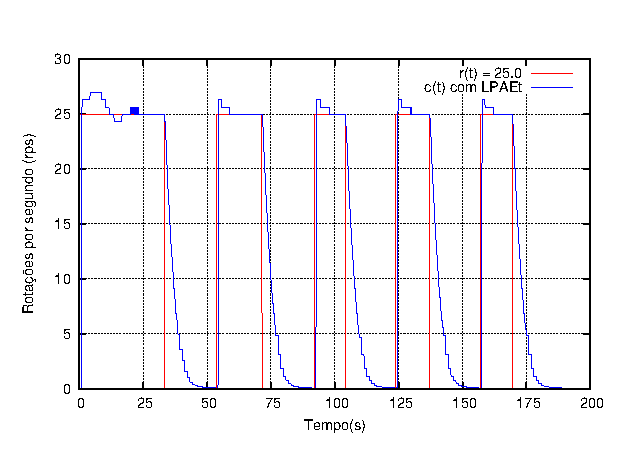
\includegraphics[scale=1.6]{./plot/LPAEt-delta.eps}
\label{fig:acaoLPAEtDelta}

{\small Fonte: Próprio autor}
\end{figure}
%%%%%%%%%%%%%%%%%%%%%%%%%%%%%%%%%%%%%%%%%%%%%%%%%%

Em outro teste, foram ajustandos os limiares,
e foi possível chegar ao resultado mostrado na Figura \ref{fig:LPAEterro}, 
onde pode-se comparar o resultado em dois momentos distintos,
no primeiro e no segundo ciclo,
comparativamente ao modelo gerado no Capítulo 3 deste trabalho.


%%%%%%%%%%%%%%%%%%%%%%%%%%%%%%%%%%%%%%%%%%%%%% Fig
\begin{figure}[!htb]%%%%%%%%%%%%%%%%%%%%%%%%%%%%%%
\caption{Erro na Ação de controle utilizando LPA$E\tau$}
\vspace{-1cm}\center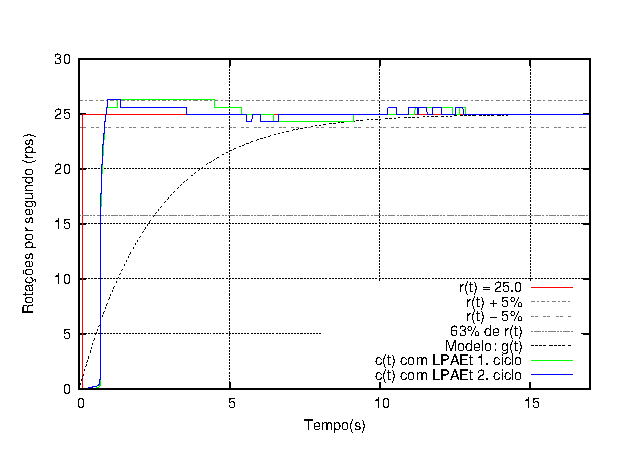
\includegraphics[scale=1.5]{./plot/LPAEt-erro.eps}
\label{fig:LPAEterro}

{\small Fonte: Próprio autor}
\end{figure}
%%%%%%%%%%%%%%%%%%%%%%%%%%%%%%%%%%%%%%%%%%%%%%%%%%

%A Figura \ref{fig:LPAEterro} mostra alguns parâmetros de 
%referência, como o valor de referência, 
%$r(t) = 25.0$ e linhas tracejadas indicando a 
%tolerância adotada como critério de desempenho de 
%$\pm $5\% além da curva do modelo do sistema.

O resultado obtido com o Controlador utilizando a 
LPA$E\tau$ proposta com o diagrama Pereira-Leão, é apresentada em dois sinais sobrepostos,
um para cada ciclo de operação, 
pois, no primeiro ciclo, a variável de correção $\delta$
ainda não foi ajustada, e a partir do segundo ciclo em diante, 
a resposta é mais rápida e mais acertiva pois já há um
valor de correção carregado, 
levando em consideração o ciclo anterior. 
Mesmo que não seja o mais adequado, 
deve ser o mais próximo do valor desejado, 
permitindo uma correção mais rápida, 
como se vê na resposta do segundo ciclo.


Pode ser destacada a redução do período em que o sistema atua
ligeiramente acima do limiar de $5\%$, consideravelmente reduzido.


Para evidenciar o ganho de performance, 
foi calculado o erro relativo percentual médio,
da mesma forma como foi realizado para obtenção do modelo
do sistema em estudo, 
apresentado neste capítulo.

A Tabela \ref{tab:ErroLPAEt} mostra
a comparação entre o primeiro e o segundo ciclo de acionamento do
sistema. Para cada ciclo foi feita a amostragem do sinal em um
intervalo que varia de 0,00s até 17,00s. A análise de cada um dos ciclos é
apresentada considerando a zona morta em uma das amostras e
desconsiderando-a em outra. Para ambos os tipos de intervalo, o erro médio
relativo cai no segundo ciclo, independente de considerar ou não a
zona morta. Mas ressalta-se que a zona morta causa um erro relativo
considerável à análise completa do sinal. Lembrando que o erro é
calculado em relação ao valor de referência $r(t)$. 
Como pode ser visto, há um ganho percentual de 
aproximadamento 1\% entre a atuação do primeiro 
para o segundo ciclo de acionamento. 



%%%%%%%%%%%%%%%%%%%%%%%%%%%%%%%%%%%%%%%%%%%%%% Tab
\begin{table}[h]%%%%%%%%%%%%%%%%%%%%%%%%%%%%%%%%%%
\centering
\caption{Erro Relativo Percentual do controlador LPA$E\tau$}
\label{tab:ErroLPAEt}

\begin{tabular}{c|c|c|c}
\hline
Ciclo de Atuação & Tipo de intervalo & Intervalo de amostras  &  erro médio relativo \\ \hline
\hline
1º & com zona morta & 0,00 a 17,00 s &  5,44 \% \\ \hline
1º & sem zona morta & 0,88 a 17,00 s &  1,90 \% \\ \hline
2º & com zona morta & 0,00 a 17,00 s &  4,41 \% \\ \hline
2º & sem zona morta & 0,88 a 17,00 s &  0,82 \% \\ \hline
\end{tabular}

{\vspace{0.2cm} \small Fonte: Próprio autor}
\end{table}
%%%%%%%%%%%%%%%%%%%%%%%%%%%%%%%%%%%%%%%%%%%%%%%%%%



%%%%%%%%%%%%%%%%%%%%%%%%%%%%%%%%%%%%%%%%%%%%%%%%%%
%%%%%%%%%%%%%%%%%%%%%%%%%%%%%%%%%%%%%%%%%%%%%%%%%%
